%----------- Necessary Style Preamble -----------%

\documentclass[mathserif, 10pt]{beamer} %

\usepackage[framesassubsections]{beamerprosper}
\usepackage{beamerthemesplit} % Activate for custom appearance
\usepackage[english]{babel}
\usepackage[latin1]{inputenc}
\usepackage{amsmath, hyperref, subfigure, multirow, rotating}
\usepackage{epstopdf}
\usepackage{verbatim}
\usepackage{listings}
\usepackage{color}
\usepackage{esint}
\usepackage{mathrsfs}
\usepackage{amsmath}


%\usepackage{enumitem}

\usetheme{Frankfurt}
\usecolortheme{default}
\usecolortheme[rgb={0.1,0.4,0.0}]{structure} % CSU color style
%\usecolortheme[rgb={0.541,0.149,0.196}]{structure} % BME color style

\setbeamersize{text margin left=0.5cm}
\setbeamersize{text margin right=0.5cm}

\setbeamercovered{transparent}

\usepackage{remreset}
\makeatletter
\@removefromreset{subsection}{section}
\makeatother
\setcounter{subsection}{1}

\makeatletter
\newcommand\xleftrightarrow[2][]{\ext@arrow 0099{\longleftrightarrowfill@}{#1}{#2}}
\def\longleftrightarrowfill@{\arrowfill@\leftarrow\relbar\rightarrow}
\makeatother


\newcommand\Wider[2][3em]{%
\makebox[\linewidth][c]{%
  \begin{minipage}{\dimexpr\textwidth+#1\relax}
  \raggedright#2
  \end{minipage}%
  }%
}

%----------- Math Definitions -----------%

\definecolor{Blue}{rgb}{0,0,1}
\def\ci{\perp\!\!\!\perp}
\def\a{\mathbf{a}}
\def\d{\mathbf{d}}
\def\e{\mathbf{e}}
\def\f{\mathbf{f}}
\def\g{\mathbf{g}}
\def\b{\mathbf{b}}
\def\q{\mathbf{q}}
\def\v{\mathbf{v}}
\def\x{\mathbf{x}}
\def\y{\mathbf{y}}
\def\u{\mathbf{u}}
%\def\z{\mathbf{\mathfrak{z}}}
\def\z{\mathbf{z}}
\def\D{\mathbf{D}}
\def\S{\mathbf{S}}
\def\X{\mathbf{X}}
\def\Z{\mathbf{Z}}
\def\1{\raisebox{.5pt}{\textcircled{\raisebox{-.9pt} {1}}}}
\def\2{\raisebox{.5pt}{\textcircled{\raisebox{-.9pt} {2}}}}
\def\3{\raisebox{.5pt}{\textcircled{\raisebox{-.9pt} {3}}}}
\def\balph{\boldsymbol\alpha}
\def\bmu{\boldsymbol\mu}
\def\btheta{\boldsymbol\theta}
\def\bomega{\boldsymbol\omega}
\def\bDelta{\boldsymbol\Delta}

%----------- Title Page Parameters -----------%
\title[Digital Control \& Digital Filters]{Digital Controls \& Digital Filters \\ Lectures 1 \& 2}
\author[M.R. Azimi]{M.R. Azimi, Professor}
\institute[CSU-ECE]{Department of Electrical and Computer Engineering \\ Colorado State University}
\date{Spring 2017}

\logo{
\includegraphics[height=0.5cm]{csu-logo.png}}

\newcommand{\unt}[1]{ \mathrm{\ #1}}

\begin{document}

%----------- slide --------------------------------------------------%

\frame{\titlepage}



\section{Digital Control Systems and Advantages}

%----------- slide --------------------------------------------------%
\frame
{

\small
\renewcommand{\theenumi}{\alph{enumi}}
\frametitle{Digital versus Analog Control Systems}

Block diagrams of typical analog and digital (sampled-data) control systems are shown below. As can be seen the plant is still analog
while the controller is replaced by a sampler (A/D converter), a digital controller (filter), and a hold device (D/A converter).


\begin{center}
\includegraphics[width=.7\linewidth]{./Figures/Analog-block.png}
\end{center}

\begin{center}
\includegraphics[width=.75\linewidth]{./Figures/Digital-block.png}
\end{center}


}

%----------- slide --------------------------------------------------%
\frame
{

\normalsize

\frametitle{Why Digital Control?}

\textcolor{blue}{\textbf{Benefits:}}\\
\begin{itemize}
%\scriptsize
\item \textit{Reduced Sensitivity and Robustness}: Unlike analog controllers digital ones are not sensitive to environmental variations and aging.
\item \textit{Better Adaptability}: Parameters of digital controllers can more easily be adapted to the changes in a changing plant i.e.
adaptive control strategies are more suited for digital control systems.
\item \textit{Form Factor}: Digital devices are more compact and lightweight comparing to their analog counterparts.
\item \textit{Cost Effectiveness}: Digital controllers are generally cheaper.
\item \textit{More Reliable}: Digital controllers are more reliable as their characteristics don't drift with time.
\end{itemize}

\textcolor{red}{\textbf{Drawback:}}\\
\begin{itemize}
\item \textit{Quantization Effects}: In designing digital systems one must be aware of the quantization effects (e.g., roundoff and truncation)
due to finite word length of the processors.
\end{itemize}
}

%----------- slide --------------------------------------------------%
\frame
{

\normalsize

\frametitle{Example}

\scriptsize Examples below show block diagrams of an autopilot system with position and rate feedback for: (a) analog control, (b) digital control,
and digital control with multirate sampling for situations where the signals have different bandwidths.

\begin{center}
\includegraphics[width=.5\linewidth,height=2in]{./Figures/Example1}
\end{center}
\vspace{-0.5in}
\begin{center}
\includegraphics[width=.5\linewidth,,height=1in]{./Figures/Example2}
\end{center}


}


\section{$z$-Transform}

%----------- slide --------------------------------------------------%
\frame
{

\frametitle{Review of $z$-Transform}

\small
The role of $z$-transform to digital systems is similar to that of Laplace transform to continuous-time systems.

\textcolor{red}{Definition 1:}   The $z$-Transform of a two-sided sequence $\{x(n)\}$ is defined by \\ \vspace{.2in}

$X(z) = \sum_{n=-  \infty}^{\infty} x(n)z^{-n}$ \\ \vspace{.2in}

If $\{x(n)\}$ is a right-sided sequence, i.e. $x(n) = 0, ~~\forall  n<0$ then \\ \vspace{.1in}
$X(z) = \sum_{n=0}^{\infty} x(n)z^{-n}$ \\ %\vspace{.2in}
\vspace{.1in}
\textcolor{red}{Example 1:}  \\
Let  $x(n) = a^n u_s(n)$, where $u_s(n)$ is the unit step function defined as, \\
\[u_s(n)= \begin{cases}
  1 & n \geq 0 \\
0 & n<0 \end{cases} \]
Find $X(z)$. \\
Using  $\sum_{n=0}^{\infty} \alpha^n=\frac{1}{1-\alpha}$ for $|\alpha|<1$, we have \\ \vspace{.1in}

$X(z) = \sum_{n=0}^{\infty} a^n z^{-n} = \sum_{n=0}^{\infty} (\frac{a}{z})^{n}=\frac{1}{1-\frac{a}{z}}=\frac{z}{z-a}$ if $|z|>a$ \\ \vspace{.7in}

}
%----------- slide --------------------------------------------------%
\frame
{
\frametitle{$z$-Transform}

\small Thus the region of convergence (ROC) for this example extends from circle with radius $a$ to $\infty$.
\begin{figure}[h]
\hspace{1.5in}
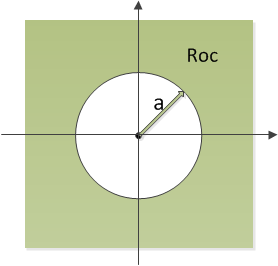
\includegraphics[width=.2\textwidth]{./Figures/roc_right_a.png}
%\caption{\label{fig:roc9} }
\end{figure}

\textcolor{red}{Example 2:} \\
Let  $ x(n) = A~sin(\Omega _0 nT)$, $\forall n \ge 0$. Find $X(z)$.  \\ \vspace{.1in}
Using Euler formula, \\
$X(z) = \sum_{n=0}^{\infty} Asin(\Omega_0 nT) z^{-n} =A \sum_{n=0}^{\infty} \frac{e^{j \Omega_0 nT}-e^{-j \Omega nT}}{2j}z^{-n}$ \\ \vspace{.1in}
$= \frac{A}{2j} \left [ \sum_{n=0}^{ \infty} (\frac{e^{j \Omega_0 T}}{z})^n - \sum_{n=0}^{ \infty} (\frac{e^{-j \Omega_0 T}}{z})^n \right ] = \frac {A}{2j} \left [ \frac{1}{1-e^{j \Omega_0 T}z^{-1}}-\frac{1}{1-e^{-j \Omega_0 T}z^{-1}} \right ]=$ \\ \vspace{.1in}
$ \frac{2Az^{-1}sin( \Omega_0 T)}{1-2z^{-1}cos( \Omega_0 T)+z^{-2}}$ exists when  $| \frac{e^{j \Omega_0 T}}{z} | <1 $ or $|z|>1 $  (since $|e^{j \Omega_0 T}|=1$)     \\ \vspace{.1in}

Thus, ROC extends from circle with radius  1 to $\infty$ similar to that of Example 1.
%\begin{figure}[h]
%\vspace{-.75in}
%
%\hspace{2.5in}
%\includegraphics[width=.1\textwidth]{./Figures/roc_right.png}
%%\caption{\label{fig:roc9} }
%\end{figure}

}


%----------- slide --------------------------------------------------%
\frame
{
\frametitle{$z$-Transform}

\textcolor{red}{Remarks:} \\ \vspace{.1in}

\begin{enumerate}
\item  For a right-sided sequence ROC is outside a circle bounded on the inside by largest magnitude pole and on the outside by $\infty$.
\item  For a left-sided sequence ROC is inside a circle bounded on the outside by smallest magnitude pole and on the inside by $0$.
\item For a two-sided sequence ROC is within a ring (between two circles) bounded on the inside by the pole with largest magnitude for $n \geq 0$ (i.e. right-sided part) and on the outside by the pole with smallest magnitude for $n < 0$.

\item \textbf{ Note:} ROC should NOT enclose a pole.

\end{enumerate}

\begin{figure}[h]
%\vspace{-.75in}

%\hspace{2.5in}
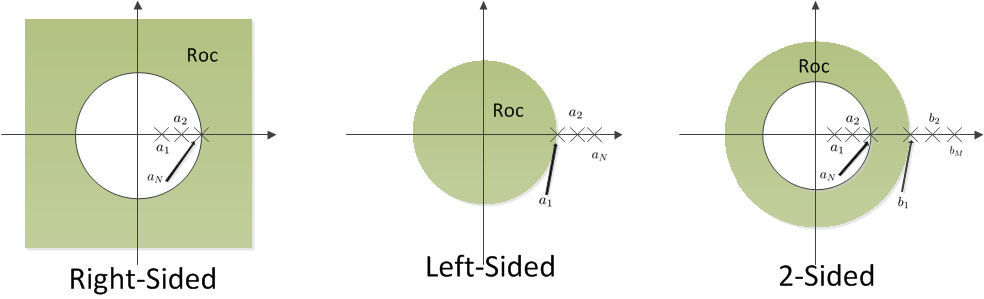
\includegraphics[width=.6\textwidth]{./Figures/roc_all.png}
%\caption{\label{fig:roc9} }
\end{figure}
 \center $a_N>...>a_2>a_1$~~~~~~~~~~~~$b_1<b_2<...<b_M$
}

\section{$z$-Transform Properties}
%----------- slide --------------------------------------------------%
\frame
{
\frametitle{Properties}
1. \textcolor{red}{ Linearity}\\ \vspace{.1in}
Let $x_1(n) \xleftrightarrow[]{z} X_1(z) $  \hspace{0.2in} ROC  $R_1<|z|<R_2$\\
\hspace{.15in} $x_2(n) \xleftrightarrow[]{z} X_2(z) $  \hspace{0.2in} ROC  $R_3<|z|<R_4$ \\ \vspace{.2in}
Then $ax_1(n)+bx_2(n) \xleftrightarrow[]{z} aX_1(z)+bX_2(z)$ \hspace{0.2in}  ROC  $R_5<|z|<R_6$ \\ \vspace{.1in}
where $R_5 = \max(R_1,R_3)$~~~~ $ R_6=\min(R_2,R_4)$ \\ \vspace{.1in}

\textcolor{red}{Remark:} \\
If linear combination leads to pole-zero cancellation, ROC may be larger. For example,
both $x_1(n)=a^n u_s(n)$ and $x_2(n)=a^n u_s(n-1)$ have ROCs $|z|>a$ but $x_1(n)-x_2(n)=\delta(n)$ has a ROC
which is the entire $z$-plane because $X_1(z)= \frac{z}{z-a}$ and $X_2(z)= \frac{a}{z-a}$ hence
$X_1(z)-X_2(z)=\frac{z-a}{z-a}=1$, i.e. ROC is everywhere.



}

%----------- slide --------------------------------------------------%
\frame
{
\frametitle{$z$-Transform Properties-Cont.}

2.  \textcolor{red}{Shift-in-Time}\\ \vspace{.1in}
Let $x(n) \xleftrightarrow[]{z} X(z) $  \hspace{0.2in} ROC  $R_1<|z|<R_2$\\ \vspace{.1in}
Then $x(n-n_0) \xleftrightarrow[]{z} z^{-n_0}X(z)$ \hspace{0.2in}  ROC  $R_1<|z|<R_2$ \\ \vspace{.1in}

Thus, ROCs are the same except possibly at $z=0$ or $z=\infty$. To see this, consider example, \\

$x_1(n) = \delta (n) \xleftrightarrow[]{z} X_1(z) = 1$ \hspace{0.2in} ROC is everywhere on $z$-plane \\
$x_2(n) = \delta(n-1) \xleftrightarrow[]{z} X_2(z) = \frac{1}{z}$ \hspace{0.2in} ROC is everywhere except at $z=0$ \\
$x_3(n) = \delta(n+1) \xleftrightarrow[]{z} X_3(z) = z$ \hspace{0.2in} ROC is everywhere except at $z = \infty$ \\ \vspace{.1in}


\textcolor{blue}{Generalizations:}\\ \vspace{.1in}
$x(n-n_0) \xleftrightarrow[]{z} z^{-n_0} \left [X(z) - \sum_{k=-n_0}^{-1}x(k)z^{-k} \right ]$ with IC's $x(-1),..,x(-n_0)$. \\ \vspace{.1in}

$x(n+n_0) \xleftrightarrow[]{z} z^{n_0} \left [X(z) - \sum_{k=0}^{n_0-1}x(k)z^{-k} \right ]\longmapsto$ More useful

}

%----------- slide --------------------------------------------------%
\frame
{
\frametitle{$z$-Transform Properties-Cont.}
3. \textcolor{red}{Multiplication by an Exponential Sequence}\\ \vspace{.1in}
Let $x(n) \xleftrightarrow[]{z} X(z) $  \hspace{0.2in}  ROC  $R_1<|z|<R_2$\\ \vspace{.1in}
Then $a^nx(n) \xleftrightarrow[]{z} X(z/a)$  \hspace{0.2in}  ROC  $|a|R_1<|z|<|a|R_2$ \\ \vspace{.1in}

Thus, ROC is scaled by $|a|$. \\ \vspace{.1in}

4. \textcolor{red}{ Differentiation}\\ \vspace{.1in}
Let $x(n) \xleftrightarrow[]{z} X(z) $  \hspace{0.2in}  ROC  $R_1<|z|<R_2$\\ \vspace{.1in}
Then $nx(n) \xleftrightarrow[]{z} -z \frac{dX(z)}{dz}$  \hspace{0.2in}  ROC  $R_1<|z|<R_2$ \hspace{0.2in} i.e. ROC is unchanged. \\ \vspace{.1in}

5.  \textcolor{red}{Conjugate (Complex Signals)}\\ \vspace{.1in}
Let $x(n) \xleftrightarrow[]{z} X(z) $  \hspace{0.2in}  ROC  $R_1<|z|<R_2$\\ \vspace{.1in}
Then $x^*(n) \xleftrightarrow[]{z}  X^*(z^*)$  \hspace{0.2in}  ROC  $R_1<|z|<R_2$  \hspace{0.2in} i.e. ROC is unchanged.

}




%----------- slide --------------------------------------------------%
\frame
{
\frametitle{$z$-Transform Properties-Cont.}

6. \textcolor{red} {Initial Value Theorem}\\ \vspace{.1in}
If $x(n) = 0~~~\forall n<0 ~~$(right-sided)\\ \vspace{.1in}
Then $x(0) =\lim_{z\to\infty} X(z)$\\ \vspace{.1in}

7.  \textcolor{red}{Final Value Theorem (FVT)} \\ \vspace{.1in}
If $x(n) = 0~~\forall n<0$ \\ \vspace{.1in}
Then $\lim_{n \to \infty} x(n) = \lim_{z \to 1} (1-z^{-1})X(z) = \lim_{z \to 1} (z-1)X(z)$ \\ \vspace{.1in}
\textbf{Condition:} As long as $(1-z^{-1})X(z)$ does not have a pole on or outside the unit circle. \\ \vspace{.1in}

\textbf{Note:} FVT is very useful for steady-state error analysis in control systems. \\ \vspace{.1in}

\textcolor{red} {Example:}\\ \vspace{.1in}
For $x(n) = sin( \Omega n)$ from Table 2.3, we have $X(z) = \frac{z~sin(\Omega)}{z^2-2zcos(\Omega ) +1}$. \\ \vspace{.08in}

Now, if we use FVT $lim_{z \to 1}(1-z^{-1})X(z) =  \lim_{z \to 1} \frac{(z-1)sin(\Omega)}{(z^2-2zcos(\Omega)+1)} = 0$.
}

%----------- slide --------------------------------------------------%
\frame
{
\frametitle{$z$-Transform Properties-Cont.}

This result contradicts with $\lim_{n \to \infty} sin( \Omega n)=? $
due to the fact that the above condition for using FVT is not satisfied since $(1-z^{-1})X(z)$ has poles on the unit circle  $z_{1,2}= e^{\pm j \Omega}$.   \vspace{.15in}


8. \textcolor{red} {Linear Convolution}\\ \vspace{.2in}
If $y(n) = x(n)*h(n)$ where $*$ stands for linear convolution operation i.e. $y(n) = x(n)*h(n)=\sum\limits_{k=- \infty}^{\infty} x(k) h(n-k) = \sum\limits_{k=- \infty}^{\infty} x(n-k)h(k)$\\
and\\
$x(n) \xleftrightarrow[]{z} X(z) $  \hspace{0.2in} ROC  $R_1<|z|<R_2$\\
$h(n) \xleftrightarrow[]{z} H(z) $ \hspace{0.2in} ROC  $R_3<|z|<R_4$\\ \vspace{.2in}
Then $Y(z) = X(z)H(z) $ \hspace{0.2in} ROC $\max[R_1,R_3]<|z|<min[R_2,R_4]$\\ \vspace{.1in}

\textbf{Note:} If a pole that borders on the ROC of one of the $z$-transforms is cancelled by a zero of the other, then the ROC of $Y(z)$ will be larger.




}



\end{document}

